\documentclass{article}
\usepackage{graphicx}
\usepackage{listings}
\usepackage{subfigure}
\usepackage{caption}

\lstset{
  language=C,
  basicstyle=\ttfamily\scriptsize,
  tabsize=2,                    % sets default tabsize to 2 spaces
%  columns=flexible,
  xleftmargin=18pt,
  xrightmargin=1em,
  numbers=left,
  numberstyle=\scriptsize,
  numbersep=1em,
  showstringspaces=false,
  alsoletter={-},
	morekeywords={todo}, %FIXIT
	otherkeywords={TD},  %FIXIT
  captionpos=b,
  escapeinside={@}{@},
  commentstyle=\color{gray},
}


\begin{document}

\author{Pavlos Katsogridakis}
\title{Malcom Docs}

\maketitle

\begin{abstract}
Malcom (Mal ALgebra Cost MOdel) is a
\end{abstract}

\section{Introduction}
\subsection{Use Cases}
\begin{enumerate}
  \item Prediction of the memory footprint
  \item Instruction ordering by the compiler
  \item Parallelism level
\end{enumerate}

\section{Instructon Grouping}

\subsection{Select}

For the range selects, to predict the size of a select instruction,
we run kNN(k=5) in our training set, considering the lower and higher bounds
as metrics. When we are facing a one bound select (<,>...) we use the
dataset statistics to fill the other bound (e.g in case of < we want the column min).
TODO subsequent selects...

\begin{figure}[t]
\begin{lstlisting}[frame=single]
  def div(i1, i2):
    return (i1.hi-i1.lo) / (i2.hi-i2.lo)

  def extrapolate(traini, testi):
      traini.cnt*div(testi,traini)*testi.approx_arg_cnt/traini.argcnt

  def predict(testi, traind, approxG):
    knn5 = traind.knn(testi,5)
    return sum([i.extrapolate(testi) for i in knn5]) / len(knn5)
\end{lstlisting}
  \caption{Code snippet for making predictions for range selects}
  \label{sel:code}
\end{figure}


\subsection{Join}
Nothing special yet

\subsection{Group}

\subsection{Set instructions}
diff,union,intersect

\subsection{Calc instructions}
Trivial to predict,
% +,*,/,- instruction produce the same result size as the input size.

\subsection{Many to One}
This category includes operations like sum, avg, min, max, single, dec\_round
The count of the result it obviously one.

\subsection{Load instructions}
\subsubsection{bind}
Bind instruction loads(or memory maps) a column into memory,
thus the result size is the size of the column.
\subsubsection{bind\_idxbat, tid}
fill this
\section{Experiments}
\subsection{Select Error for tpch-sf-10}

\subsection{Whole query evaluation}

\begin{figure}[ht]
  \centering
  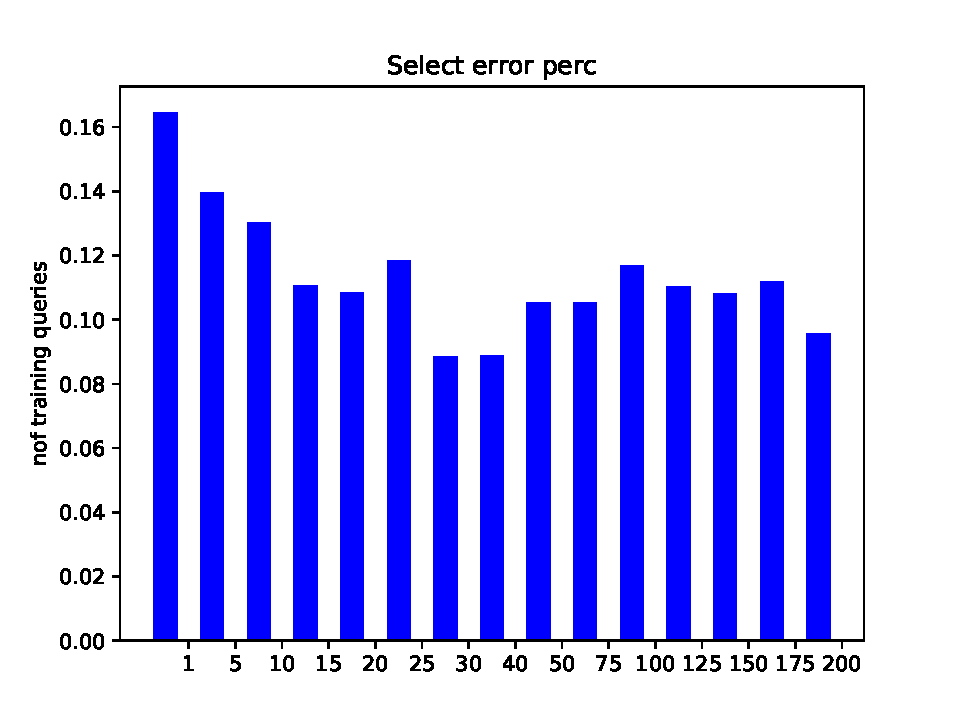
\includegraphics[scale=0.7]{figs/select_error_q6.pdf}
  \caption{Query 6 selection error}
  \label{fig:sel6}
\end{figure}

\end{document}
